% Rain Barrel Pump System – Product Test Report
% ------------------------------------------------
\documentclass[12pt]{article}

% PAGE LAYOUT & HEADER/FOOTER
\usepackage[margin=1in]{geometry}
\setlength{\headheight}{14.5pt}             % for fancyhdr
\usepackage{fancyhdr}
\fancyhf{}
\fancyhead[L]{USC Facilities: Rain Barrel Water Pump System}
\fancyfoot[C]{\thepage}

% TABLES, MATH, LISTS, GRAPHICS, CODE
\usepackage{booktabs}
\usepackage{longtable}
\usepackage{amsmath}
\usepackage{enumitem}
\usepackage{graphicx}
\usepackage{array}
\usepackage{hyperref}
\usepackage{xcolor}
\usepackage{setspace}
\usepackage{titlesec}
\usepackage{listings}
  \lstset{
    basicstyle=\ttfamily\small,
    breaklines=true,
    frame=single,
    backgroundcolor=\color{gray!10},
    keywordstyle=\bfseries,
  }
\usepackage{siunitx}
\usepackage{caption}
\usepackage{pdflscape}

% Setup header
\pagestyle{fancy}
\fancyhf{}
\fancyhead[L]{USC Facilities: Rain Barrel Water Pump System} % Team name in the header
\fancyfoot[C]{\thepage} % Page number in the footer


\begin{document}


%------------------------------------------------
% COVER PAGE
%------------------------------------------------
\title{
  \vspace{2in}
  \textbf{EMCH428-002} \\[1ex]
  \textbf{Product Testing Report} \\[1ex]
  \textbf{Sponsor: USC Facilities} \\[1ex]
  \vspace{2in}
}
\author{
  \textbf{Team Members:} \\[2ex]
  Tanner Harmon\\[1ex]
  Presston McConnell\\[1ex]
  William Wenzel\\[1ex]
  JC Vaught\\[2ex]
}
\date{}
\maketitle
\thispagestyle{fancy}

\newpage
\setcounter{page}{2}

%================================================
% 1. Introduction
%================================================
\section*{1. Introduction}
\begin{itemize}[leftmargin=*]
  \item This report details the verification testing of a solar‐compatible pump that pressurizes water from a 1000 gal rain barrel for campus irrigation.
\end{itemize}

\subsection*{1.1 Target and Fallback Specifications}
\begin{table}[h]
  \centering
  \caption*{Table 1 -- Product Target and Fallback Specifications}
  \begin{tabular}{@{}clcc@{}}
    \toprule
    \# & Need / Engineering Characteristic & Target & Fallback \\
    \midrule
    1 & Flow rate              & 12–16 gpm & 8–12 gpm \\
    2 & Outlet pressure        & 40–60 psi & 20–40 psi \\
    3 & Annual energy cost     & $<$\$50 yr$^{-1}$ & $<$\$150 yr$^{-1}$ \\
    4 & Durability             & $\ge10\,\mathrm{yr}$ & $\ge5\,\mathrm{yr}$ \\
    5 & Ease of assembly       & $<5\,\mathrm{h}$ & $<8\,\mathrm{h}$ \\
    6 & Capital cost           & $<$\$2{,}000 & $<$\$2{,}500 \\
    7 & Safety (GFCI + relief) & Pass \& relief $<75$ psi & Pass \& relief $<80$ psi \\
    \bottomrule
  \end{tabular}
\end{table}

\subsection*{1.2 Parameters Directly Tested}
\begin{itemize}[leftmargin=*]
  \item Flow rate
  \item Outlet pressure
  \item Energy consumption (annualized cost)
  \item Electrical \& pressure safety (GFCI, relief valve)
\end{itemize}

\subsection*{1.3 Parameters \emph{Not} Directly Tested}
\begin{itemize}[leftmargin=*]
  \item Durability – long‐term exposure evaluation scheduled; prototype < 1 month old.
  \item Ease of assembly – timing to be captured during final production build.
  \item Capital cost – final BOM awaiting invoice completion.
\end{itemize}

\newpage
%================================================
% 2. Test Methods
%================================================
\section*{2. Test Methods}
The protocols below are formatted so they are easily reproducible.

\subsection*{2.1 Parameter 1 – Flow Rate}
\begin{itemize}[leftmargin=*]
  \item \textbf{Target / fallback:} 12–16 gpm / 8–12 gpm
  \item \textbf{Equipment / Instrumentation:} 5‑gal graduated bucket (0.25 gal marks); modern smartphone (120 fps); stopwatch backup.
  \item \textbf{Methodology:}
    \begin{enumerate}[label=\arabic*., leftmargin=*]
      \item Verify ≥ 200 gal of water in rain collection tank.
      \item Ensure the pump is powered (solar or mains).
      \item Place hose inside bucket; start video (or stopwatch) at spigot opening.
      \item Record timestamps every 0.5 gal up to 5 gal.
      \item Repeat until pump cycles off at cut‐off pressure.
    \end{enumerate}
  \item \textbf{Direct measurements:} Video‐derived fill times (s) and gauge pressure.
  \item \textbf{Calculations / analyses:}
    \[
      Q = \frac{V}{t}, 
      \quad
      u = \frac{s}{\sqrt{n}},
    \]
    where $s$ is the sample standard deviation (computed in Python).
\end{itemize}

\subsection*{2.2 Parameter 2 – System Pressure}
\begin{itemize}[leftmargin=*]
  \item \textbf{Target / fallback:} 40–60 psi / 20–40 psi
  \item \textbf{Equipment:} 0–100 psi inline gauge; smartphone camera.
  \item \textbf{Methodology:} Film the gauge during a flow run.
  \item \textbf{Measurements:} Pause video, read pressure.
  \item \textbf{Calculations:} Mean, σ, uncertainty as above.
\end{itemize}

\subsection*{2.3 Parameter 3 – Energy Cost}
\begin{itemize}[leftmargin=*]
  \item \textbf{Target / fallback:} $<$\$50 yr$^{-1}$ / $<$\$150 yr$^{-1}$
  \item \textbf{Equipment:} Fluke 373 clamp meter; Kill‑A‑Watt; solar controller logs.
  \item \textbf{Procedure:}
    \begin{enumerate}[label=\arabic*., leftmargin=*]
      \item Mount watt‐meter at pump inlet; enable log on charge controller.
      \item Run one 270 s cycle; record $P_{\mathrm{surge}}$, $P_{\mathrm{steady}}$; repeat 3×.
      \item Extract daily runtime $t_{\mathrm{daily}}$ (h/day) from logs.
    \end{enumerate}
  \item \textbf{Measurements:} $P_{\mathrm{surge}}$ (W), $P_{\mathrm{steady}}$ (W), cycle time (s), $t_{\mathrm{daily}}$ (h/day).
  \item \textbf{Calculations:}
    \[
      E_{\mathrm{annual}}
        = \frac{P_{\mathrm{steady}}\times t_{\mathrm{daily}}\times365}{1000}
        \quad(\mathrm{kWh/yr}),
      \quad
      \text{Cost}
        = E_{\mathrm{annual}}\times\$0.1294.
    \]
\end{itemize}

\subsection*{2.4 Parameter 4 – Safety (GFCI / Pressure Relief)}
\begin{itemize}[leftmargin=*]
  \item \textbf{Specs:}
    \begin{itemize}[leftmargin=1.5em]
      \item \textbf{GFCI:} Must trip within 30 ms at $\le5\,\mathrm{mA}$ ground‑fault current (Target \& Fallback both require pass).
      \item \textbf{Relief valve:} Opens < 75 psi (Target) / < 80 psi (Fallback).
    \end{itemize}
  \item \textbf{Equipment:}
    \begin{itemize}[leftmargin=1.5em]
      \item GFCI tester (Ideal SureTest 61‑164)  
      \item Calibrated relief valve (70 psi setpoint)  
      \item Auxiliary \SI{0.75}{hp} pump  
      \item Inline 0–100 psi gauge (± 1 psi)  
      \item Smartphone (120 fps)
    \end{itemize}
  \item \textbf{Setup:}
    \begin{enumerate}[label=\arabic*., leftmargin=*]
      \item Gauge upstream of relief valve.  
      \item Camera viewing gauge + valve.
      \item Pump on GFCI circuit.
    \end{enumerate}
  \item \textbf{Procedure:}
    \begin{enumerate}[label=\arabic*., leftmargin=*]
      \item Inject 5 mA fault; confirm breaker trips/resets.  
      \item With main pump off, pressurize at ~5 psi/min until valve opens; record.  
      \item Reseat, repressurize, repeat 3×.
    \end{enumerate}
  \item \textbf{Measurements:} GFCI pass/fail; $P_{\mathrm{open},i}$ (psi), $i=1\ldots3$.
  \item \textbf{Calculations:} $\bar P_{\mathrm{open}},\,s,\,u=s/\sqrt{3}$, compare to limits.
\end{itemize}

% ================================================================
% 3. Analysis
% ================================================================
\newpage
\section*{3\; Analysis}

\subsection*{3.1\; Flow Rate Results}
\begin{itemize}[leftmargin=*]
  \item \textbf{Python code:}
    \begin{lstlisting}[language=Python]
import statistics, math
flow_rates = [...]  # 120 measurements
Q_mean = statistics.mean(flow_rates)
s_Q = statistics.stdev(flow_rates)
u_Q = s_Q / math.sqrt(len(flow_rates))
print(Q_mean, s_Q, u_Q)
    \end{lstlisting}
  \item \textbf{Equations:}
    \[
      \bar Q = \frac{1}{N}\sum_{i=1}^N Q_i,\quad
      s_Q = \sqrt{\frac{1}{N-1}\sum_{i=1}^N (Q_i - \bar Q)^2},\quad
      u_Q = \frac{s_Q}{\sqrt{N}}
    \]
  \item \textbf{Results:} $\bar Q = 12.14$ gpm, $s_Q = 1.30$ gpm, $u_Q = 0.12$ gpm ($N=120$)
  \item \textbf{Outcome:} Meets fallback (8 gpm).
\end{itemize}

\subsection*{3.2\; Outlet Pressure Results}
\begin{itemize}[leftmargin=*]
  \item \textbf{Python code:}
    \begin{lstlisting}[language=Python]
psis = [...]  # 120 readings
P_mean = statistics.mean(psis)
s_P = statistics.stdev(psis)
u_P = s_P / math.sqrt(len(psis))
print(P_mean, s_P, u_P)
    \end{lstlisting}
  \item \textbf{Equations:}
    \[
      \bar P = \frac{1}{N}\sum_{i=1}^N P_i,\quad
      s_P = \sqrt{\frac{1}{N-1}\sum_{i=1}^N (P_i - \bar P)^2},\quad
      u_P = \frac{s_P}{\sqrt{N}}
    \]
  \item \textbf{Results:} $\bar P = 32.24$ psi, $s_P = 6.25$ psi, $u_P = 0.57$ psi ($N=120$)
  \item \textbf{Outcome:} Fallback satisfied; below target (40 psi).
\end{itemize}

\subsection*{3.3\; Relief‑Valve Results}
\begin{itemize}[leftmargin=*]
  \item \textbf{Python code:}
    \begin{lstlisting}[language=Python]
relief = [71, 76, 68]
mean_r = statistics.mean(relief)
s_r = statistics.stdev(relief)
u_r = s_r / math.sqrt(len(relief))
print(mean_r, s_r, u_r)
    \end{lstlisting}
  \item \textbf{Equations:}
    \[
      \bar P_{\mathrm{open}} = \frac{1}{n}\sum_{i=1}^n P_i,\quad
      s = \sqrt{\frac{1}{n-1}\sum_{i=1}^n (P_i - \bar P_{\mathrm{open}})^2},\quad
      u = \frac{s}{\sqrt{n}}
    \]
  \item \textbf{Results:} $\bar P_{\mathrm{open}} = 71.7$ psi, $s = 4.0$ psi, $u = 2.3$ psi ($n=3$)
  \item \textbf{Outcome:} Target met (<75 psi).
\end{itemize}

\subsection*{3.4\; Energy Cost Results}
\begin{itemize}[leftmargin=*]
  \item \textbf{Python code:}
    \begin{lstlisting}[language=Python]
P = 1314       # steady draw in W
t_daily = 270/3600  # cycle time in h
E_year = P * t_daily * 365 / 1000
cost = E_year * 0.1294
print(E_year, cost)
    \end{lstlisting}
  \item \textbf{Equations:}
    \[
      E_{\mathrm{annual}}
        = \frac{P \times t_{\mathrm{daily}} \times 365}{1000},\quad
      \text{Cost}
        = E_{\mathrm{annual}} \times 0.1294
    \]
  \item \textbf{Results:} $E = 35.99$ kWh/yr, Cost = \$4.32/yr
  \item \textbf{Outcome:} Target met.
\end{itemize}


% ================================================================
% 4. Conclusions / Recommendations
% ================================================================
\newpage\section*{4. Conclusions / Recommendations}
\begin{table}[h]
  \centering
  \caption{Summary of Measured Performance}
  \begin{tabular}{@{}lcccc@{}}
    \toprule
    Parameter      & Target           & Fallback        & Measured             & Sat.? \\
    \midrule
    Flow rate      & 12--16 gpm       & 8--12 gpm       & 12.14 ± 0.12 gpm       & Y     \\
    Pressure       & 40--60 psi       & 20--40 psi      & 32.24 ± 0.57 psi     & Y (FB)
    \\
    Energy cost    & $<$\$50/yr         & $<$\$150/yr       & 4.32/yr              & Y     \\
    Durability     & \multicolumn{2}{c}{see text} & Not tested            & N     \\
    Ease of assembly & \multicolumn{2}{c}{see text} & Not tested            & N     \\
    Capital cost   & $<$\$2000          & $<$\$2500         & Pending               & N     \\
    Safety         & GFCI / $<$75 psi   & GFCI / $<$80 psi  & Pass                  & Y     \\
    \bottomrule
  \end{tabular}
\end{table}

\subsection*{4.1 Parameters Not Meeting Requirements}
\begin{itemize}[leftmargin=*]
  \item \textbf{Durability:} Long-term testing incomplete.
    \begin{itemize}[leftmargin=*]
      \item \emph{Plan:} Quarterly inspections \& accelerated weather chamber exposure.
    \end{itemize}
  \item \textbf{Ease of assembly:} Build time not recorded.
    \begin{itemize}[leftmargin=*]
      \item \emph{Plan:} Build a similar system; measure the time taken to build. The time taken to build this prototype is likely in the weeks.
    \end{itemize}
  \item \textbf{Capital cost:} Some hardware not procured.
    \begin{itemize}[leftmargin=*]
      \item \emph{Plan:} Finalize BOM; leverage surplus stores to finish construction.
    \end{itemize}
\end{itemize}

\subsection*{4.2 Overall Assessment}
Prototype \emph{is satisfactory}. All tested criteria meet at least fallback. 

\subsection*{4.3 Next-Step Recommendations}
\begin{itemize}[leftmargin=*]
  \item Initiate durability cycle and record assembly timing.
  \item Re-evaluate HOQ after modifications to ensure no secondary trade-offs.
\end{itemize}

% ================================================================
% 5. Appendix
% ===============================================================



% … later in the document …          % only if you need extra width
\newpage \subsection*{Appendi}
\begin{small}
\begin{longtable}{S[table-format=3.2] S[table-format=2.1] S[table-format=2.0]}
\caption{Time (s), Cumulative Volume (gal), and Outlet Pressure (psi)}\\
\toprule
{Time (s)} & {Total Gallon} & {PSI} \\
\midrule
\endfirsthead
\multicolumn{3}{c}{\tablename\ \thetable{} -- continued}\\
\toprule
{Time (s)} & {Total Gallon} & {PSI} \\
\midrule
\endhead
\midrule
\multicolumn{3}{r}{\footnotesize Continued on next page}\\
\endfoot
\bottomrule
\endlastfoot
0.00  &  0.0 & 40 \\
4.35  &  0.5 & 39 \\
8.80  &  1.0 & 38 \\
13.35 &  1.5 & 37 \\
17.90 &  2.0 & 37 \\
22.55 &  2.5 & 36 \\
27.20 &  3.0 & 35 \\
31.95 &  3.5 & 34 \\
36.70 &  4.0 & 34 \\
41.55 &  4.5 & 33 \\
46.40 &  5.0 & 32 \\
51.35 &  5.5 & 32 \\
56.35 &  6.0 & 31 \\
61.40 &  6.5 & 31 \\
66.50 &  7.0 & 30 \\
71.65 &  7.5 & 29 \\
76.85 &  8.0 & 29 \\
82.15 &  8.5 & 28 \\
87.45 &  9.0 & 28 \\
92.80 &  9.5 & 27 \\
98.25 & 10.0 & 27 \\
103.75 & 10.5 & 26 \\
109.25 & 11.0 & 26 \\
114.85 & 11.5 & 25 \\
120.50 & 12.0 & 25 \\
126.25 & 12.5 & 24 \\
132.00 & 13.0 & 24 \\
137.80 & 13.5 & 23 \\
143.70 & 14.0 & 23 \\
149.65 & 14.5 & 23 \\
155.65 & 15.0 & 22 \\
161.70 & 15.5 & 22 \\
167.80 & 16.0 & 21 \\
174.00 & 16.5 & 21 \\
180.20 & 17.0 & 21 \\
186.50 & 17.5 & 20 \\
192.85 & 18.0 & 20 \\
199.15 & 18.5 & 21 \\
205.25 & 19.0 & 22 \\
211.20 & 19.5 & 23 \\
217.05 & 20.0 & 24 \\
222.75 & 20.5 & 25 \\
228.35 & 21.0 & 26 \\
233.85 & 21.5 & 27 \\
239.25 & 22.0 & 28 \\
244.60 & 22.5 & 28 \\
249.80 & 23.0 & 29 \\
255.00 & 23.5 & 30 \\
260.10 & 24.0 & 31 \\
265.15 & 24.5 & 31 \\
270.10 & 25.0 & 32 \\
275.05 & 25.5 & 33 \\
279.90 & 26.0 & 33 \\
284.75 & 26.5 & 34 \\
289.55 & 27.0 & 34 \\
294.30 & 27.5 & 35 \\
299.00 & 28.0 & 35 \\
303.70 & 28.5 & 36 \\
308.35 & 29.0 & 36 \\
313.00 & 29.5 & 36 \\
317.60 & 30.0 & 37 \\
322.20 & 30.5 & 37 \\
326.75 & 31.0 & 37 \\
331.30 & 31.5 & 37 \\
335.85 & 32.0 & 38 \\
340.35 & 32.5 & 38 \\
344.85 & 33.0 & 38 \\
349.35 & 33.5 & 38 \\
353.85 & 34.0 & 38 \\
358.30 & 34.5 & 39 \\
362.80 & 35.0 & 39 \\
367.25 & 35.5 & 39 \\
371.70 & 36.0 & 39 \\
376.10 & 36.5 & 39 \\
380.55 & 37.0 & 39 \\
385.00 & 37.5 & 39 \\
389.40 & 38.0 & 39 \\
393.85 & 38.5 & 39 \\
398.25 & 39.0 & 40 \\
402.65 & 39.5 & 40 \\
407.10 & 40.0 & 40 \\
411.50 & 40.5 & 40 \\
415.90 & 41.0 & 40 \\
420.30 & 41.5 & 40 \\
424.70 & 42.0 & 40 \\
429.10 & 42.5 & 40 \\
433.50 & 43.0 & 40 \\
437.85 & 43.5 & 40 \\
442.25 & 44.0 & 40 \\
446.65 & 44.5 & 40 \\
451.05 & 45.0 & 40 \\
455.45 & 45.5 & 40 \\
459.80 & 46.0 & 40 \\
464.20 & 46.5 & 40 \\
468.60 & 47.0 & 40 \\
473.00 & 47.5 & 39 \\
477.45 & 48.0 & 38 \\
482.00 & 48.5 & 38 \\
486.55 & 49.0 & 37 \\
491.15 & 49.5 & 36 \\
495.85 & 50.0 & 35 \\
500.55 & 50.5 & 34 \\
505.35 & 51.0 & 34 \\
510.15 & 51.5 & 33 \\
515.05 & 52.0 & 32 \\
520.00 & 52.5 & 32 \\
525.00 & 53.0 & 31 \\
530.00 & 53.5 & 31 \\
535.10 & 54.0 & 30 \\
540.25 & 54.5 & 29 \\
545.50 & 55.0 & 29 \\
550.75 & 55.5 & 28 \\
556.05 & 56.0 & 28 \\
561.45 & 56.5 & 27 \\
566.85 & 57.0 & 27 \\
572.35 & 57.5 & 26 \\
577.85 & 58.0 & 26 \\
583.45 & 58.5 & 25 \\
589.10 & 59.0 & 25 \\
594.80 & 59.5 & 24 \\
600.00 & 60.0 & 24 \\
\end{longtable}
\end{small}


\newpage 
\begin{figure}[htbp]
  \centering
  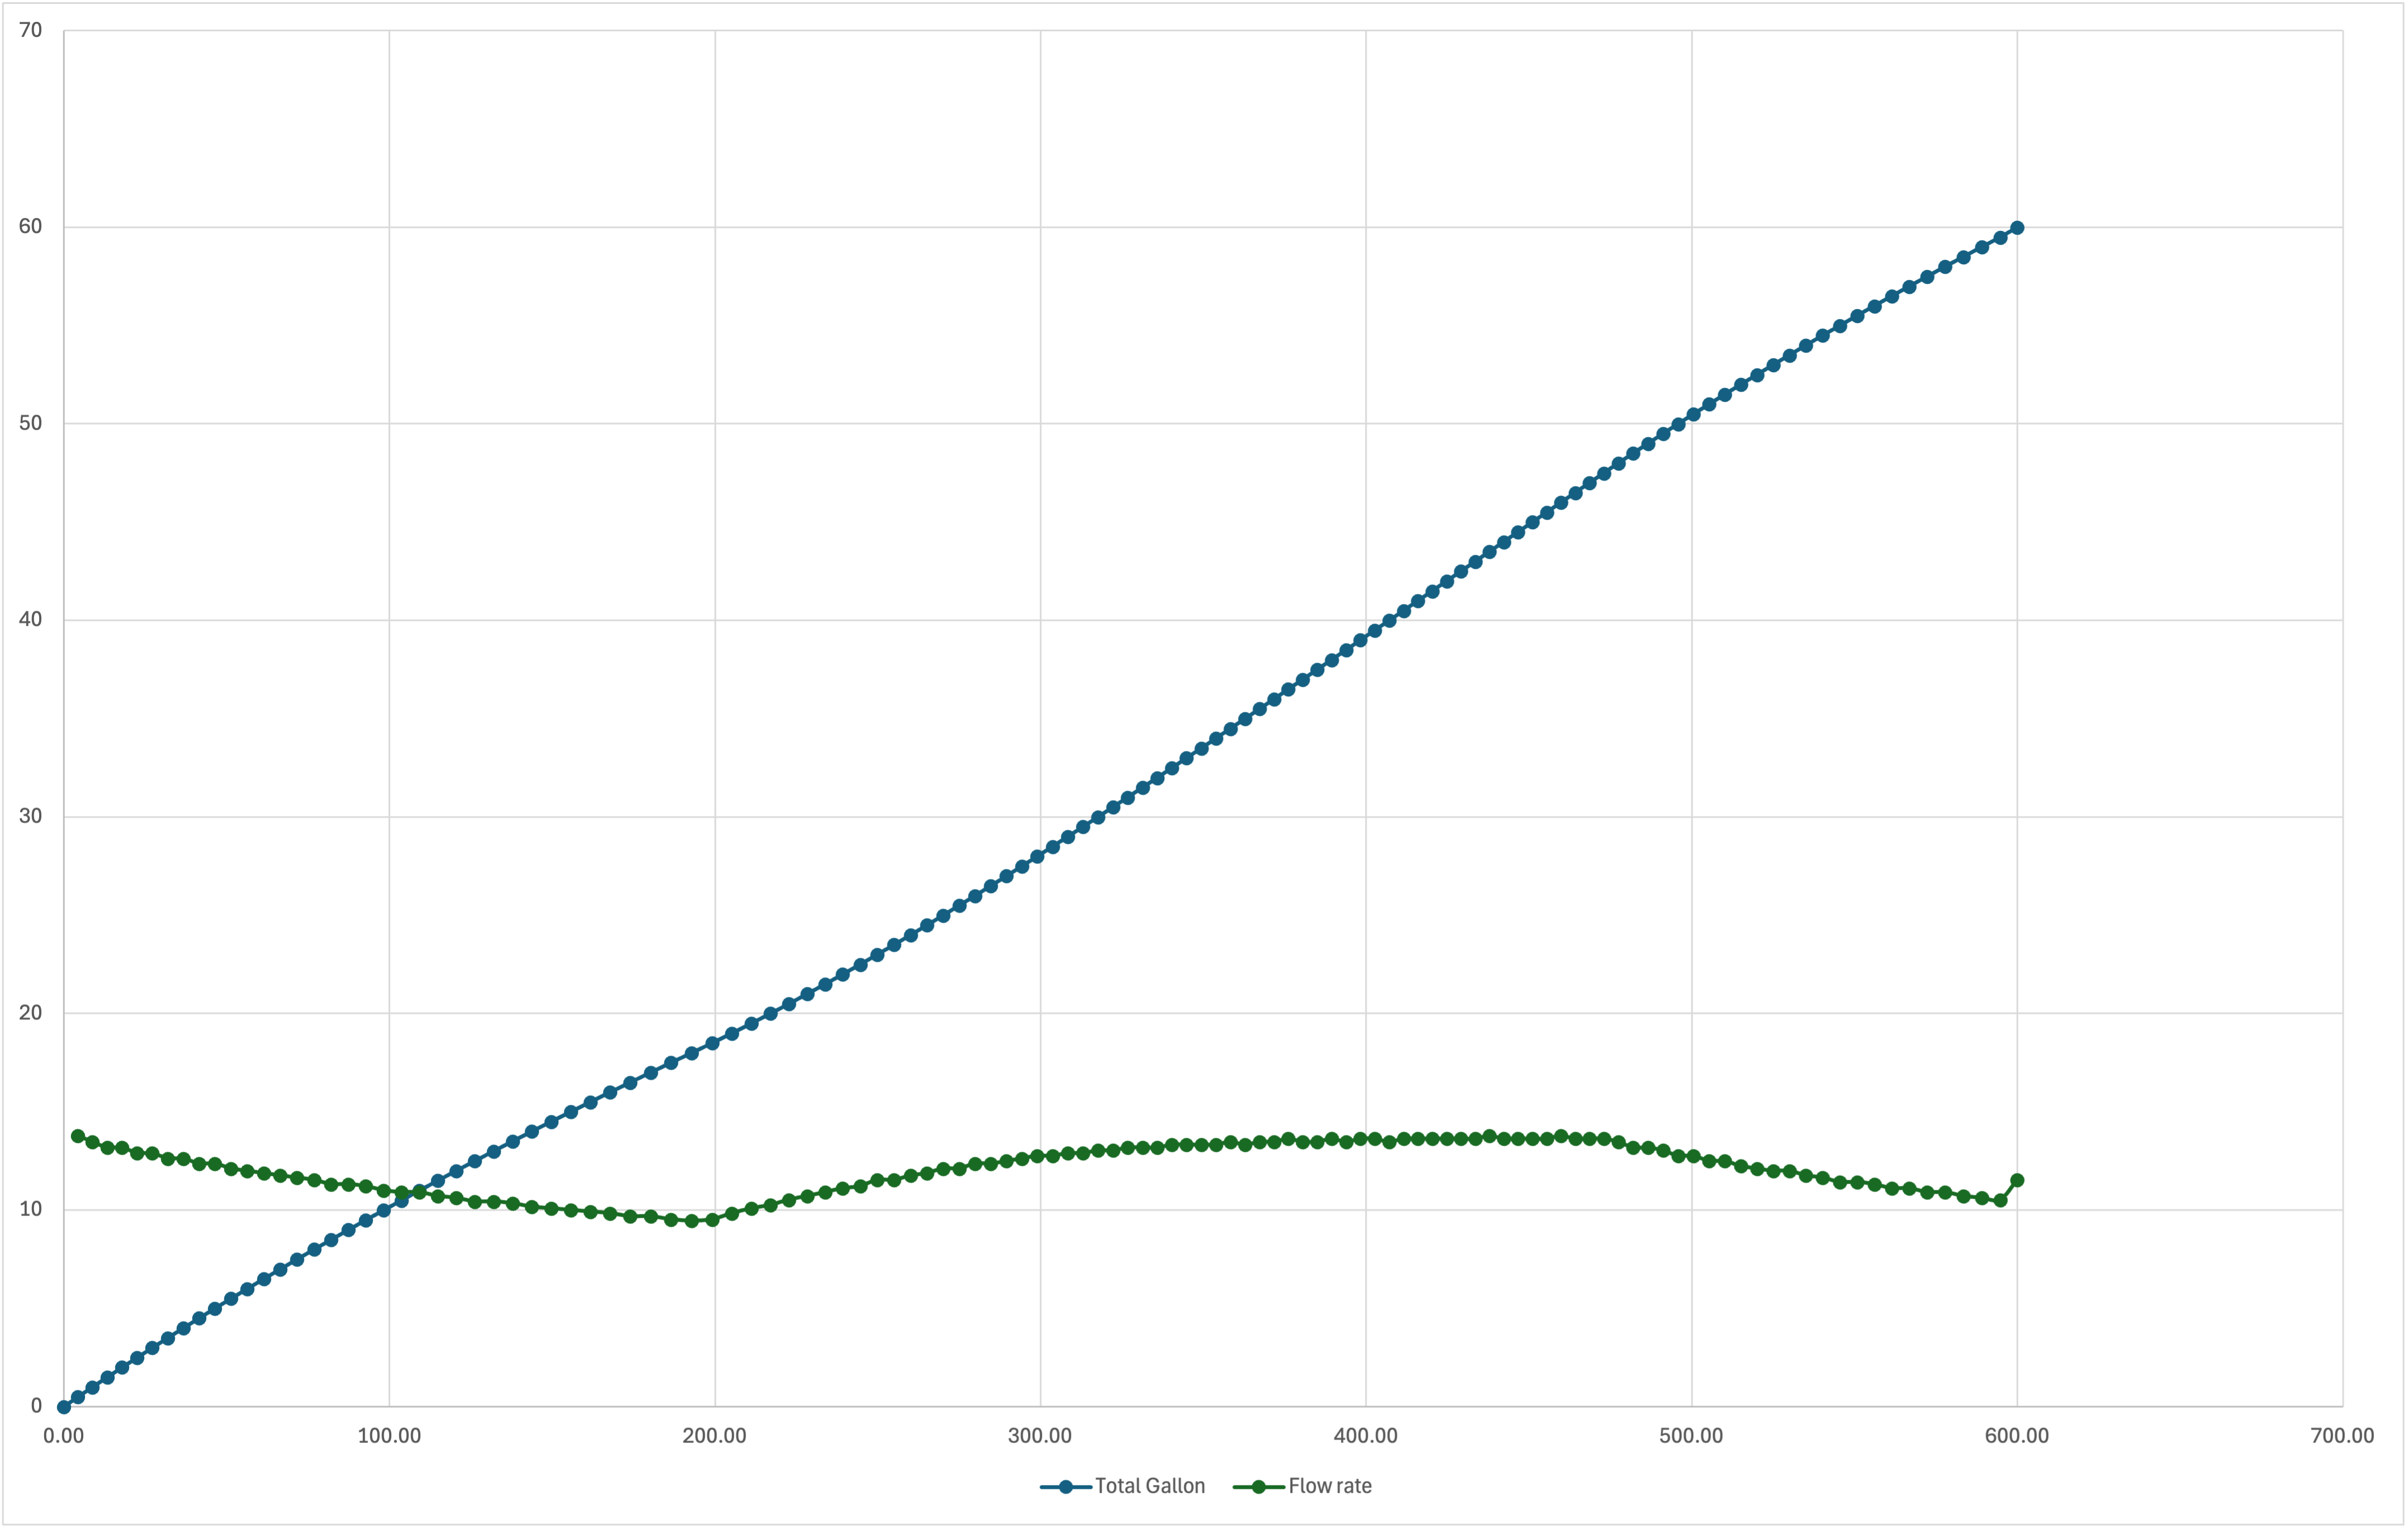
\includegraphics[width=0.8\textwidth]{flowrate.png}
  \caption{Instantaneous flow rate (gpm) and cumulative volume (gallon) vs.\ time}
  \label{fig:flowrate}
\end{figure}

\begin{figure}[htbp]
  \centering
  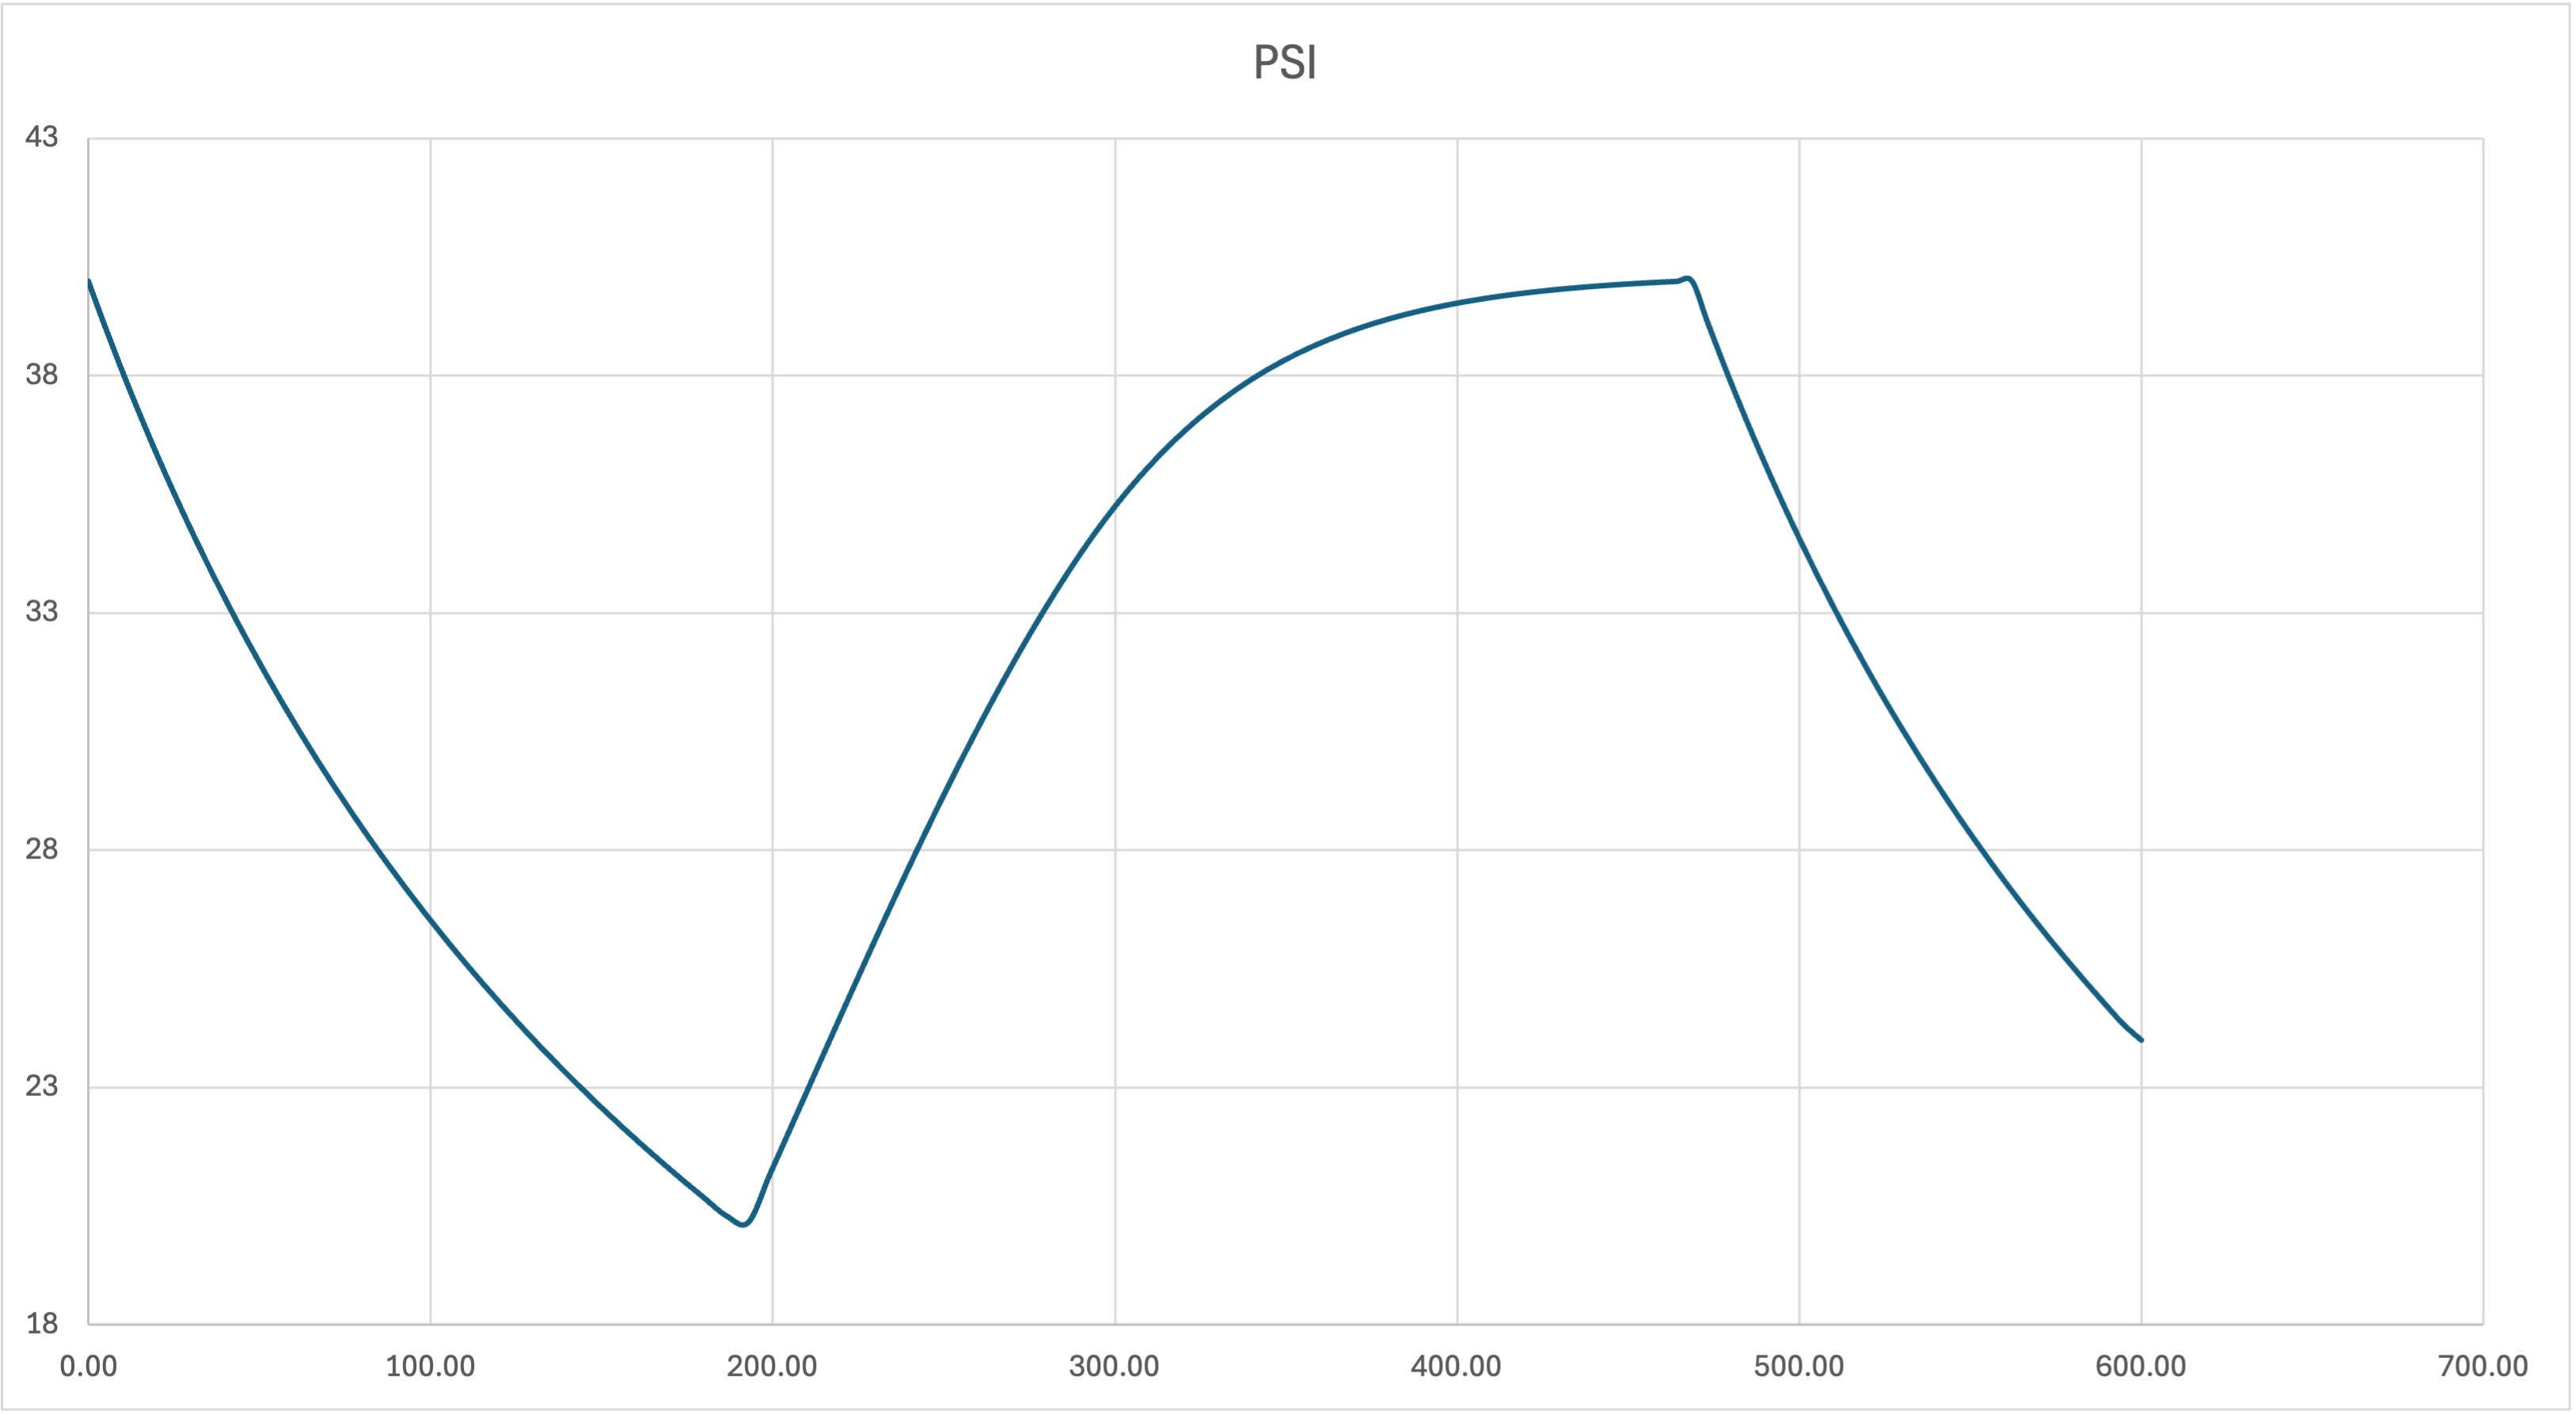
\includegraphics[width=0.8\textwidth]{pressure.png}
  \caption{Smoothed pressure (\si{psi}) vs.\ time (\si{s}).}
  \label{fig:pressure}
\end{figure}


\end{document}
